\documentclass{article}
\PassOptionsToPackage{numbers,sort&compress}{natbib}
\PassOptionsToPackage{portrait}{geometry}
\usepackage[preprint]{neurips_2026}
\makeatletter
\renewcommand{\@noticestring}{MD6329 Deep Learning for Healthcare AI}
\makeatother
\usepackage[utf8]{inputenc}
\usepackage[T1]{fontenc}
\usepackage{amsmath,amsfonts,booktabs,graphicx,microtype,url,xcolor}
\usepackage{placeins}
\usepackage{hyperref}
\graphicspath{{figures/}}
\raggedbottom
\setcounter{topnumber}{3}
\setcounter{bottomnumber}{2}
\setcounter{totalnumber}{5}
\renewcommand{\topfraction}{0.9}
\renewcommand{\bottomfraction}{0.8}
\renewcommand{\textfraction}{0.08}
\setlength{\textfloatsep}{12pt plus 2pt minus 2pt}
\setlength{\floatsep}{10pt plus 2pt minus 2pt}
\hypersetup{colorlinks=true,linkcolor=blue,citecolor=blue,urlcolor=blue,pdftitle={PharmaScan: Calibrated Open Set Pill Verification}}
\title{PharmaScan: Calibrated Open Set Pill Verification\\with Visual Embeddings and Imprint Evidence}
\author{Ding Zixin\\Nanyang Technological University\\Student ID: G2602715D\And Pan Shengxin\\Nanyang Technological University\\Student ID: G2601614B}
\begin{document}
\setcounter{page}{1}
\maketitle
\setlength{\parskip}{3.5pt}
\begin{abstract}
For patients managing several medicines, verification of loose pills involves recognising newly enrolled medicines while rejecting pills outside a personal medication list. PharmaScan formulates this task as retrieval from a personal gallery, with explicit outcomes for an accepted match, an unknown pill and a request for another photograph. A hybrid visual encoder is trained with an angular margin objective to produce a 256-dimensional embedding, through which each medicine is enrolled from three photographs without network retraining. Rejection and ambiguity thresholds are selected using separate validation medicines, while optical character recognition with Florence-2 supplies complementary imprint evidence. On 200 held-out appearance groups from the Computational Photography Project for Pill Identification (C3PI) collection, simulated galleries of ten medicines yield 76.0\% correct naming and 0.04\% wrong naming among enrolled queries, with 94.8\% rejection of medicines outside the gallery. Imprint re-ranking increases identification accuracy among 4,936 catalogue products from 71.6\% to 80.2\%. Transfer to MEDISEG reveals a substantial acquisition gap, with 70.4\% of enrolled queries rejected as unknown. These findings support calibrated verification under familiar imaging conditions and identify acquisition shift and imprint visibility as constraints on broader use.
\end{abstract}

\section{Introduction}
\label{sec:problem}
Verification of loose tablets and capsules is a practical challenge in medication management because removal from packaging separates a medicine from its identifying information. Appearance then provides a recognition cue, although orientation, illumination and the visible side vary, and similar colours and shapes occur across products and strengths. Within the problem of medication errors addressed by the World Health Organization's Medication Without Harm initiative~\citep{who2017medication}, visual verification concerns the association between a photographed pill and a known medicine before a medication decision is made.

A personal medication list creates an evolving recognition task in which newly prescribed medicines are enrolled from a few photographs and a query may belong to none of the enrolled identities. Recognition therefore depends on a representation that transfers across identities, together with a decision rule that distinguishes a plausible match from an unfamiliar or ambiguous pill. Since an incorrect accepted name and a request for further checking have different consequences, retrieval accuracy alone provides an incomplete account of verification performance. Existing pill retrieval benchmarks support representation learning~\citep{usuyama2020epillid,ling2020fewshot}, while the personal workflow additionally involves membership rejection and handling of close candidates.

PharmaScan formulates this task as retrieval from a personal gallery with three outcomes: an accepted identity, \textsc{unknown}, or \textsc{retake}. Medicines are registered through a shared visual embedding without network retraining, and decisions combine similarity to the nearest enrolment prototype with separation from the next candidate. Optical character recognition (OCR) using \mbox{Florence-2}~\citep{xiao2024florence2} supplies complementary imprint evidence, while catalogue retrieval provides candidates when matching within the personal gallery is insufficient. Product name and strength remain associated with the pharmacy label~\citep{moh_medication_label}, as visual similarity alone does not establish strength or suitability for administration.

The study investigates verification of previously unseen medicines from three enrolment photographs at an operating point selected on validation data, with particular attention to accepted misidentification, imprint evidence and acquisition transfer. Evaluation combines a strict identity-disjoint test from the National Library of Medicine (NLM) Computational Photography Project for Pill Identification (C3PI) collection~\citep{yaniv2016nlm}, the ePillID benchmark~\citep{usuyama2020epillid}, and MEDISEG images of Hong Kong products~\citep{mediseg2026}. Their respective protocols, detailed in Section~\ref{sec:setup}, distinguish transfer to new identities under familiar conditions from changes in cameras, product population and scene. The project plan's validation targets and corresponding measurements are reported separately from held-out results in Appendix~\ref{app:calibration}, Table~\ref{tab:targets}.

The contribution is a calibrated verification workflow and an empirical analysis of the effects of its design choices. Sequential training changes, imprint re-ranking and rejected reader adaptations are examined through accepted errors and abstention, revealing acquisition shift as a constraint even when misidentification among enrolled queries is rare. The evidence is drawn from public image datasets and simulated galleries, with patient outcomes outside the evaluation scope.

\section{Related Work}
\label{sec:related}
\paragraph{Pill identification and low-shot retrieval.}
Consumer-to-reference matching was established as a medication recognition task by the NLM Pill Image Recognition Challenge~\citep{yaniv2016nlm}, followed by fine-grained pill identification using learned convolutional features and comparisons with handcrafted descriptors~\citep{wong2017pill}. These studies demonstrate the usefulness of appearance while exposing the difficulty of separating similar products under image variation within a product. This setting is developed further by ePillID, whose strongest low-shot baseline combines bilinear features with multi-head metric learning~\citep{usuyama2020epillid}. Its analysis of confusing classes is relevant to personal galleries containing medicines with similar appearances, although ranked retrieval from product references leaves gallery membership rejection as a separate decision. PharmaScan evaluates both tasks and distinguishes results under strict and official protocols because access to references for test identities changes the information available during representation learning.

\paragraph{Multiple visual cues and feature fusion.}
Complementary visual cues are useful when discriminating pill characteristics are not equally visible across images. Ling et al. introduce CURE images with varied acquisition conditions, a segmentation network and a multi-stream recognition model trained using Batch All followed by Batch Hard mining~\citep{ling2020fewshot}. Their combination of pill cues and difficult training examples relates to the broader problem of recognition beyond familiar photographs. In PharmaScan, convolutional neural network (CNN) features~\citep{simonyan2015vgg} are combined with vision transformer (ViT) features~\citep{dosovitskiy2021vit}, bringing together local spatial structure and self-attention between image patches~\citep{vaswani2017attention}. These complementary spatial assumptions also connect the architecture with the course treatment of vision transformers~\citep[p.~36]{md6329lecture09}. Channel and spatial attention are provided by the Convolutional Block Attention Module (CBAM)~\citep{woo2018cbam}, while capsule routing aggregates branch features through agreement~\citep{sabour2017capsules}. The inherited architecture supplies the representation in Section~\ref{sec:arch}, whose performance is evaluated within the complete verification workflow.

\paragraph{Metric learning for enrolment.}
Similarity representations separate enrolment from network training by mapping identity information to a space used for retrieval. FaceNet learns this geometry through triplet supervision~\citep{schroff2015facenet}, while CosFace and ArcFace impose margins in cosine and angular space, respectively~\citep{wang2018cosface,deng2019arcface}. These objectives relate identity supervision to distances between examples, connecting with the course discussion of embedding geometry and matching views~\citep[pp.~38, 47--49]{md6329lecture08}. PharmaScan uses ArcFace during training and prototypes during inference, allowing the deployed gallery to contain identities outside the training classifier. Balanced identity sampling~\citep{hermans2017triplet} and evaluation protocol~\citep{musgrave2020reality} are relevant to interpreting such embeddings because optimisation and sampling changes can affect apparent differences between objectives. Accordingly, the sequential analysis in Section~\ref{sec:ablations} evaluates the combined training recipe without isolating an advantage attributable to the loss alone.

\paragraph{Open set decisions and confidence calibration.}
Open set recognition extends discrimination among known identities with a membership decision~\citep{scheirer2013openset}, for which score-based detection provides a baseline~\citep{hendrycks2017baseline}. Membership in PharmaScan is defined by the patient's enrolled gallery, so a medicine familiar to the encoder can still be foreign to the patient. The consequences of false acceptance motivate selection of the operating point on validation data and separate reporting of abstention, consistent with the course treatment of decision thresholds~\citep[p.~92]{md6329lecture02}. Calibration concerns the relationship between reported probabilities and observed correctness: Guo et al. document poorly calibrated network confidence and examine post-processing corrections~\citep{guo2017calibration}. Here, logistic calibration~\citep{platt1999probabilistic} is fitted to catalogue retrieval evidence, while gallery rejection and ambiguity retain their own thresholds. These distinct purposes underlie the decision mechanisms in Sections~\ref{sec:decision} and~\ref{sec:identify}.

\paragraph{Imprint evidence and acquisition transfer.}
Florence-2 represents multiple visual tasks through a common prompted model and supplies the pretrained imprint reader used here~\citep{xiao2024florence2}. Hidden, small or debossed text limits the evidence available to this reader, while adaptation introduces a further distinction between text recovery and verification performance. Low-rank adaptation (LoRA) provides a parameter-efficient mechanism for adapting pretrained models~\citep{hu2022lora}, but an incorrect token can promote a visually similar product even when average recovery improves. The analysis of reader adaptation therefore measures accepted identities alongside recovered text. Acquisition transfer is examined with MEDISEG, which adds instance annotations for Hong Kong products photographed under conditions different from the US reference collection~\citep{mediseg2026,chu2026mediseg}. Changes in scale, scene and product population extend the evaluation beyond retrieval within the source dataset to the transfer of both representation and calibrated decisions.

\FloatBarrier
% ===================================================================================================================
% Section: Approach (25%). Needs: amsmath, booktabs, graphicx, natbib (the NeurIPS style loads it);
% \graphicspath{{figures/}}; references.bib. Numbers: epills/configs/stage2_run4.yaml, outputs/runs/stage2_run4/.
% ===================================================================================================================
\section{Method}
\label{sec:approach}

A detected pill is cropped, embedded by a hybrid CNN and ViT encoder, and compared by cosine similarity with the
patient's enrolled medicines or with a product catalogue. Decision thresholds are calibrated on validation medicines
only, and the OCR imprint reader adds complementary evidence.

The implementation adapts the team's facial expression code (\texttt{FER/}) in the project repository\footnote{\url{https://github.com/398-21/ultrasound_Model}} and the ePillID benchmark code\footnote{\url{https://github.com/usuyama/ePillID-benchmark}}. Development and report preparation are documented in Appendix~\ref{app:development}.

\subsection{Network}
\label{sec:arch}

The encoder in Figure~\ref{fig:arch} processes each $224{\times}224$ crop through a VGG16 branch~\citep{simonyan2015vgg} with CBAM channel and spatial attention~\citep{woo2018cbam} and a ViT-B/16 branch~\citep{dosovitskiy2021vit}. Local texture, colour and edge features from the CNN are combined with the ViT's global layout representation through capsule routing~\citep{sabour2017capsules}. Each branch is projected to a 256-dimensional capsule, and initially equal coupling coefficients are updated towards the branch whose features agree with the fused vector. A small transformer encoder~\citep{vaswani2017attention} then refines four 64-dimensional tokens derived from this vector, after which their mean is mapped by a linear head to the unit-length embedding $\mathbf{z}=f_\theta(x)\in\mathbb{R}^{256}$. Auxiliary heads predict shape and colour during training. The full layer configuration, pretrained checkpoints and initialisation are given in Appendix~\ref{app:configuration}, Table~\ref{tab:arch}.

\begin{figure}[!htbp]
  \centering
  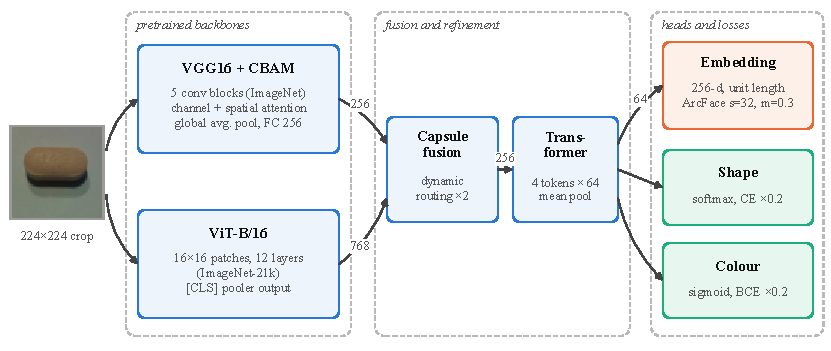
\includegraphics[width=0.98\linewidth,height=0.28\textheight,keepaspectratio]{fig02_architecture.pdf}
  \caption{The hybrid network. VGG16 with CBAM attention and ViT-B/16 see the same crop. A capsule block fuses their
    features by dynamic routing and a transformer block refines the result into a unit-length 256-d embedding trained
    with ArcFace, with auxiliary shape and colour heads. Numbers on the arrows are feature sizes.}
  \label{fig:arch}
\end{figure}



\subsection{Training}
\label{sec:training}

\paragraph{Objective.} The embedding is trained with ArcFace~\citep{deng2019arcface} over the 1,710 training
appearance groups defined in Section~\ref{sec:setup}, plus auxiliary losses:
\begin{equation}
  \mathcal{L}=-\log\frac{e^{s\cos(\theta_y+m_a)}}{e^{s\cos(\theta_y+m_a)}+\sum_{j\neq y}e^{s\cos\theta_j}}
  +\lambda_s\mathcal{L}_{\text{shape}}+\lambda_c\mathcal{L}_{\text{colour}},
  \label{eq:loss}
\end{equation}
with $s=32$, $m_a=0.3$ and $\lambda_s=\lambda_c=0.2$, where $\theta_j$ is the angle between $\mathbf{z}$ and the $j$-th
class weight, $\mathcal{L}_{\text{shape}}$ is a cross-entropy and $\mathcal{L}_{\text{colour}}$ a binary cross-entropy
(unknown labels ignored). The margin warms up over the first three epochs ($0, 0.1, 0.2$), then stays at $0.3$.

\paragraph{Optimisation.} Training follows the schedule with two phases in Table~\ref{tab:train}: the ViT and VGG blocks 1--3 are frozen during phase 1, allowing the new layers to adapt before all parameters are fine-tuned in phase 2. Each batch contains $P$ groups with $K=4$ photographs per group~\citep{hermans2017triplet}, and AdamW~\citep{loshchilov2019adamw} uses separate learning rates for pretrained backbones, new layers and the randomly initialised ArcFace class table. This separation accommodates their different initialisations, while margin warm-up introduces angular separation progressively. The combined effect of these choices is evaluated in Section~\ref{sec:ablations}.

\begin{table}[!htbp]
  \caption{Training settings of the served model (run 4). Selection: top-1 on medicines in the validation enrolment partition (best:
    phase 2, epoch 35). Seed 2026.}
  \label{tab:train}
  \centering
  \small
  \begin{tabular}{@{}lll@{}}
    \toprule
    Setting & Phase 1 & Phase 2 \\
    \midrule
    Trainable & all but ViT, VGG blocks 1--3 & all \\
    Max.\ epochs; batch ($P\times K$) & 25; $32\times4$ & 35; $16\times4$ \\
    Learning rate: backbones / new / ArcFace & $3\!\times\!10^{-5}$ / $3\!\times\!10^{-5}$ / $10^{-3}$
      & $10^{-5}$ / $10^{-5}$ / $10^{-4}$ \\
    Optimiser & AdamW, weight decay $10^{-3}$ & same \\
    Rate schedule & reduce on plateau ($\times0.5$, patience 3) & same \\
    Early stopping & patience 6, best weights restored & same \\
    \bottomrule
  \end{tabular}
\end{table}

\paragraph{Augmentation.} Colour jitter is kept small (saturation 0.05, hue 0.0125) because colour contributes to identity. Crop windows are jittered by $\times0.75$--$1.35$ with centre shifts up to 10\% to model detector error. Acquisition perturbations include brightness and contrast changes ($\pm0.3$), white balance ($\pm8\%$), downscaling to 40--160 pixels ($p=0.3$), JPEG quality 30--90 ($p=0.3$), and Gaussian noise ($\sigma=0.03$, $p=0.2$). A neighbouring pill is partly pasted into the frame with probability 0.2.

\subsection{Open-set decision rule and calibration}
\label{sec:decision}

A patient enrols each medicine $j$ from $k{=}3$ photos. Its prototype is
$\mathbf{p}_j=\sum_i f_\theta(x_{j,i})/\lVert\sum_i f_\theta(x_{j,i})\rVert$. For a query with similarities
$s_j=\mathbf{z}^\top\mathbf{p}_j$, sorted $s_{(1)}\ge s_{(2)}$,
\begin{equation}
  \hat y=\begin{cases}
    \textsc{unknown} & s_{(1)}<\tau,\\
    \textsc{retake} & s_{(1)}\ge\tau \text{ and } s_{(1)}-s_{(2)}<m,\\
    \arg\max_j s_j & \text{otherwise,}
  \end{cases}
  \label{eq:decision}
\end{equation}
where \textsc{retake} requests another photograph with the pill turned over. Calibration uses validation medicines in 1,000 simulated ten-medicine galleries, yielding $\tau=0.895$ for 95\% rejection of foreign medicines and $m=0.115$ as the largest margin with at most 10\% retakes. The crop window is selected as $1.55\times$ the detected box's long side from a sweep of 1.3--2.0, across which correct naming varies by approximately one percentage point (Figure~\ref{fig:calib}b).



\subsection{Identification with imprints and calibrated confidence}
\label{sec:identify}

For catalogue identification, a pill outside the personal gallery is ranked against 4,936 US products using each product's similarity to its closest reference as its appearance score $s$. Florence-2-large~\citep{xiao2024florence2} reads the imprint zero-shot at
four rotations (Florence-2-base for inference on a central processing unit (CPU)). Each recorded imprint token receives an inverse document frequency (IDF) weight in $[0,1]$, assigning greater weight to rare tokens such as `EC5' than to common tokens such as `93', which appears on hundreds of Teva pills. A product's imprint
score $r$ is the weight of its best token found in the reads, and the top $K{=}100$ products by look are re-ranked by
$s+\alpha r$ with $\alpha=0.05$, both chosen on validation (Figure~\ref{fig:identify}b). In the patient's gallery, only
tokens that distinguish the enrolled imprints from each other confirm or contradict a match. Catalogue confidence is estimated by logistic calibration~\citep{platt1999probabilistic} from the top candidate's appearance score, its separation from the runner-up and its imprint evidence. 

Raw cosine similarities are not probabilities: even products outside the catalogue can obtain similarities around 0.93. The fitted catalogue confidence is
\begin{equation}
  \sigma\!\left(-12.50+12.50s_1+72.13(s_1-s_2)+3.92r_1\right),
\end{equation}
where $s_1$ and $s_2$ are the appearance scores of the first two re-ranked products and $r_1$ is the first product's imprint score. This estimate concerns correctness of catalogue candidates, while gallery membership and ambiguity remain governed by Equation~\ref{eq:decision}.

\subsection{Implementation and reproducibility}
Training uses PyTorch~\citep{paszke2019pytorch} 2.11 and Hugging Face Transformers 5.19 on one NVIDIA RTX 4080 SUPER graphics processing unit (GPU) with 16\,GB memory. The deployed model is served through FastAPI on a Hugging Face ZeroGPU Space\footnote{\url{https://davidpansx-pharmascan-api.hf.space/ui/}}. Split generation, training, calibration and evaluation are separate scripts. The execution commands and output conventions are provided in Appendix~\ref{app:development}.

\subsection{Software 3.0 in coding and evaluation}
\label{sec:sw3-approach}\label{sec:sw3-experiments}
The evaluation harness was written with the coding agent from specifications in natural language, covering patient simulation, look-alike stress tests and comparisons of products from the same manufacturer, top-$k$ and confidence evaluation, figure generation, and the API's 92 tests. Testing and review identified defects including an error in the label reader that linked an extended-release sticker to the immediate-release product, which was corrected by enforcing the release form. Procedural safeguards comprised selection of settings on validation data, one evaluation of each test set, and files generated by scripts as the source of reported numerical results.

\FloatBarrier
% ===================================================================================================================
% Section: Experiments (25%). Needs: amsmath, booktabs, graphicx, natbib; \graphicspath{{figures/}}; references.bib.
% Every figure and table sits in this section, next to the text that cites it.
% Sources: epills/outputs/runs/*/eval/*.json, docs/stage2_results.md, docs/evidence.md.
% ===================================================================================================================
\section{Experiments}
\label{sec:experiments}

\subsection{Data and evaluation setup}
\label{sec:setup}

\paragraph{Training source and identity units.}
The primary source is the National Library of Medicine (NLM) Computational Photography Project for Pill Identification (C3PI) collection~\citep{yaniv2016nlm}. Its consumer-image list contains 40,882 entries, including 295 exact repeats, leaving 40,587 distinct photographs that were successfully cropped and assigned to partitions. Pill types are defined by nine-digit National Drug Code (NDC9) and product part, giving 2,400 types after package variants are consolidated. Types sharing recorded imprint, shape, colour and size form an \emph{appearance group}, while those without imprint text remain separate. The resulting 2,338 groups define training labels and partition membership, with product identities retained for catalogue retrieval.

Consumer photographs vary in illumination, orientation, visible side and background, with a median of 15 images per medicine and a range of 3--101 in the inventory's NDC9 summary. Studio references provide more consistent views for catalogue matching and augment training groups in runs 3 and 4. Appendix~\ref{app:data} details the count reconciliation, package variants and grouping process, together with the distribution plot in Figure~\ref{fig:data-statistics}.

\begin{table}[!htbp]
\centering\small
\caption{C3PI partitions after removal of repeated entries and successful cropping of all 40,587 distinct consumer photographs. Studio references add 6,198 training crops in runs 3 and 4.}
\label{tab:data}
\begin{tabular}{@{}lrrl@{}}
\toprule
Partition & Groups & Crops & Role \\
\midrule
Training & 1,710 & 29,471 & Representation learning \\
Validation enrolled & 214 & 3,556 & Selection and enrolment \\
Validation unknown & 214 & 3,555 & Rejection calibration \\
Held-out test & 200 & 4,005 & Evaluation on unseen groups \\
\bottomrule
\end{tabular}
\end{table}

\paragraph{Partitioning and preprocessing.}
Groups containing an ePillID fold-4 holdout identity are reserved through NDC9 matching. Remaining groups are randomly divided approximately 80:10:10 between training and the two validation partitions (Table~\ref{tab:data}). Code for split generation checks shared identifiers, exact duplicates and near-duplicate crops. Only references for training groups are added in runs 3 and 4. Each detected pill is framed in a square window of 1.55 times the long side of its bounding box and resized to $224\times224$ pixels. VGG16 inputs use ImageNet channel statistics, while ViT inputs are scaled to $[-1,1]$, with constants given in Appendix~\ref{app:configuration}. Training augmentation is specified in Section~\ref{sec:training}. Figure~\ref{fig:examples} provides representative views.



\begin{figure}[!htbp]
\centering
\begin{minipage}[t]{0.48\linewidth}
\vspace{0pt}\centering
\textbf{(a) C3PI image variation}\\[3pt]
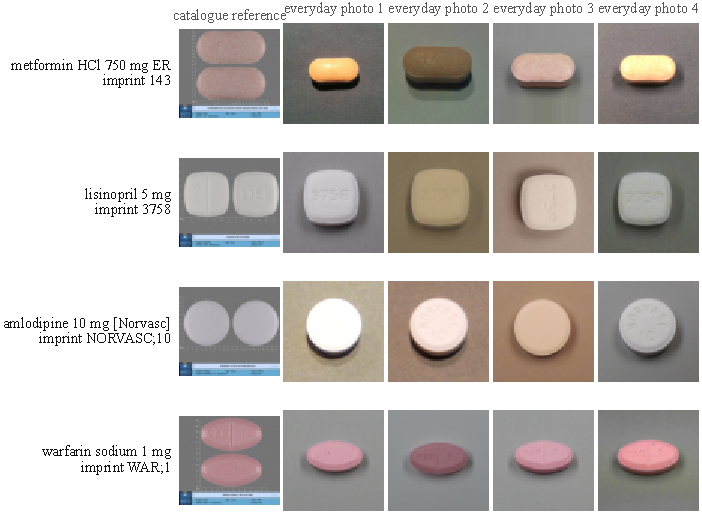
\includegraphics[width=\linewidth]{fig04_qualitative_examples.pdf}
\end{minipage}\hfill
\begin{minipage}[t]{0.49\linewidth}
\vspace{0pt}\centering
\textbf{(b) ePillID side coverage}\\[3pt]
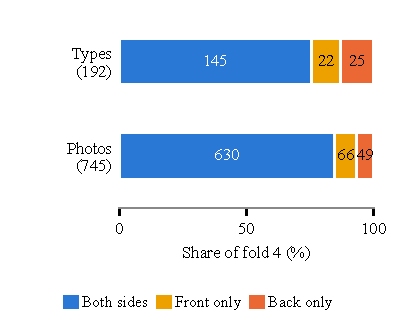
\includegraphics[width=\linewidth]{figD4_epillid_sides_compact.pdf}
\end{minipage}
\caption{Data characteristics. (a) Catalogue references and four consumer photographs for each of four medicines illustrate variation in orientation, visible side and illumination. (b) ePillID fold-4 coverage by side availability, shown for pill types and photographs.}
\label{fig:examples}
\end{figure}

\paragraph{Evaluation sources and catalogue.}
The C3PI holdout comprises 200 appearance groups, whereas the local ePillID release contains 13,532 images of 4,902 types, including 9,804 references and 3,728 consumer images. Fold 4 contains 745 consumer photographs of 192 identities~\citep{usuyama2020epillid}. The official ePillID protocol permits reference images for test types during training, distinguishing it from the strict C3PI evaluation. MEDISEG~\citep{mediseg2026} contributes 8,261 images with 14,069 annotated pills from 32 Hong Kong products. For evaluation with all products enrolled, three single-pill photographs per product form the gallery, leaving 13,973 query pills after 96 enrolment instances are excluded. The median pill long side is 81 pixels, with fifth and 95th percentiles of 27 and 194 pixels in $640\times640$ images. A separate deployment subset has 40 query pills. Product population, scale, cameras and clutter change together, so the external gap cannot be attributed to camera hardware alone. Catalogue identification uses 4,936 US products assembled from C3PI reference images and imprint, shape and colour metadata.

\paragraph{Data use.}
The study uses public image datasets without patient records. C3PI images are restricted to research and development, including when accessed through ePillID, whose MIT code licence does not supersede the image conditions. MEDISEG is distributed under CC BY 4.0, and download instructions for all sources are provided in \texttt{epills/docs/datasets.md}.


\paragraph{Metrics for medication verification.} We simulate patients with 10 enrolled medicines (3 photos each). For the
patient's own pills we report the share \emph{named correctly}, \emph{named wrongly} (an accepted misidentification),
\emph{retake} and \emph{called unknown}; for pills that are not theirs, the share \emph{rejected}. An accepted name can inform subsequent action, whereas unknown and retake outcomes add a further checking step to the workflow. We also report top-$k$ accuracy, area under the receiver operating characteristic curve (AUROC),
ePillID's mean average precision (MAP) and global average precision (GAP), and the reliability of the stated confidence. Intervals are obtained from 1,000 bootstrap replicates, resampling medicine groups with replacement and
retaining all their repeated query appearances. The 2.5th and 97.5th percentiles define the reported 95\% intervals.

\paragraph{Gallery simulation.} The evaluation code samples 1,000 galleries using seed 0. Within each
gallery, ten eligible medicines are sampled without replacement and three enrolment images are selected per
medicine. All remaining images of those medicines are used as enrolled queries. Enrolment images are excluded
from queries within that gallery. Up to 200 images of medicines outside the gallery are sampled without
replacement as foreign queries. Identities and photographs can recur across galleries. Percentages are computed
by pooling query rows rather than averaging gallery percentages. For MEDISEG, enrolment is restricted to
single-pill images. The simulation and bootstrap procedures are implemented in
\texttt{epills/src/epills/training/eval/openset.py}; they were inspected for this report.

\paragraph{Baselines.} (i) Run 1: the same network with a common recipe (new layers at $10^{-3}$, no margin
warm-up). (ii) The published ePillID models~\citep{usuyama2020epillid}. (iii) Look only versus look plus imprint, for
the gallery and the catalogue.

\subsection{Main results}
\label{sec:main}

Table~\ref{tab:main} reports results under the strict protocol. In the conditions
it was trained for, the served model (run 4) names 76.0\% of a patient's own pills correctly and only 0.04\% wrongly
(95\% confidence interval 0.02--0.07\%), while rejecting 94.8\% of pills that are not the patient's (Figure~\ref{fig:openset}a). The
imprint check raises correct names to 78.3\% (wrong 0.06\%) by settling retakes. These rates of wrong naming use enrolled queries as their denominator. With the imprint
pipeline, 3.5\% of foreign queries receive an accepted gallery identity and 94.8\% are called unknown;
the remainder request a retake (approximately 1.7\%, inferred from rounded reported rates). Thus the
0.06\% error among enrolled queries is not the overall rate of accepting a wrong medicine. Catalogue identification improves from 71.6\% to 80.2\% top-1 and from 91.7\% to 94.4\% top-5 with imprint re-ranking. Adding training-group references in run 3 raises strict ePillID MAP@1 from 13.7\% to 37.1\%. Run 4's acquisition augmentation gains 6.4 percentage points on MEDISEG while reducing C3PI top-1 by 1.2 points. Run 4 is the served model.

\begin{table}[!htbp]
  \caption{Test results on medicines never seen in training (\%; 10-medicine galleries, 3 enrolment photos,
    calibrated $\tau$ and $m$). Bottom block: the served pipeline with imprint reading (GPU reader, CPU reader in
    brackets).}
  \label{tab:main}
  \centering
  \small
  \begin{tabular}{@{}lccc@{}}
    \toprule
    & Run 2 & Run 3 & Run 4 (served) \\
    \midrule
    C3PI held-out: top-1 among 200 medicines & 82.0 & \textbf{84.4} & 83.2 \\
    \quad gallery: named correctly / wrongly & 78.6 / 0.1 & \textbf{80.4} / 0.0 & 76.0 / 0.04 \\
    \quad other medicines rejected & 94.2 & 94.1 & \textbf{94.8} \\
    MEDISEG: top-1 among 32 products & 38.9 & 41.8 & \textbf{48.2} \\
    \quad gallery: named correctly / wrongly & 17.6 / 1.1 & 18.7 / 1.0 & 18.7 / \textbf{0.7} \\
    \quad own called unknown / other rejected & 51.5 / 78.7 & 64.2 / 89.3 & 70.4 / \textbf{93.1} \\
    ePillID strict (no test type in training): MAP@1 & 13.7 & 37.1 & \textbf{42.3} \\
    \midrule
    C3PI gallery + imprint check: named correctly / wrongly & & & 78.3 (77.3) / 0.06 \\
    \quad retake / called unknown & & & 7.2 / 14.5 \\
    \quad foreign: unknown / accepted match & & & 94.8 / 3.5 \\
    Catalogue (4,936 products) + imprint: top-1 / top-5 & & & 80.2 (79.2) / 94.4 \\
    \quad look only: top-1 / top-5 & & & 71.6 / 91.7 \\
    \bottomrule
  \end{tabular}
\end{table}

\begin{figure}[!htbp]
  \centering
  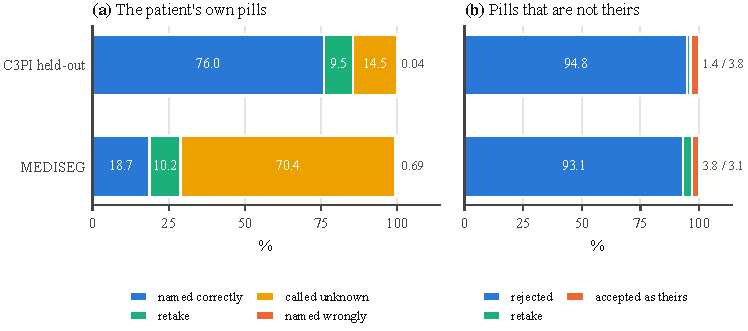
\includegraphics[width=\linewidth]{fig08_open_set_outcomes.pdf}
  \caption{What the patient sees (run 4, embedding only, 10 medicines, 3 enrolment photos). Small shares are listed
    after each bar in legend order. In C3PI conditions most own pills are named correctly and wrong names are rare;
    under acquisition shift the threshold transfers poorly and most own pills are called unknown, which limits useful recognition.}
  \label{fig:openset}
\end{figure}

\subsection{Ablations and hyperparameters}
\label{sec:ablations}

Sequential design changes are summarised in Appendix~\ref{app:calibration}, Table~\ref{tab:ablation}. The combined optimisation changes produce the largest observed improvement. With the new layers at
$10^{-3}$ the embedding collapses to about 3 effective dimensions and validation top-1 stalls at 77\%, while the revised recipe
keeps 12--15 dimensions and reaches 98\% (Figure~\ref{fig:training}). Effective dimensionality is defined as $\exp(-\sum_i q_i\log q_i)$,
where $q_i$ is the fraction of embedding variance along principal direction $i$. It equals 256 for equal variance
and one for a single direction. The decision settings are smooth
(Figure~\ref{fig:calib}): the crop window moves correct names by under one point, and the margin trades correct names
for retakes almost one for one. The imprint weight has a clear optimum (Figure~\ref{fig:identify}b), because a large
$\alpha$ lets false OCR reads promote wrong products. The imprint helps most when the pill's own imprint is actually
read: the correct product ranks first in 92.9\% of those queries, compared with 68.6\% when it is not (Figure~\ref{fig:identify}a).







\begin{figure}[!htbp]
  \centering
  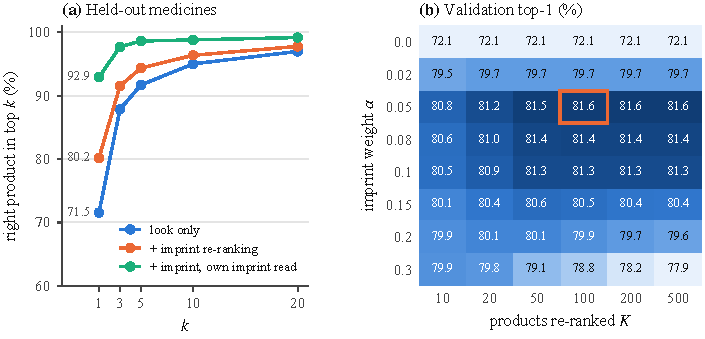
\includegraphics[width=0.92\linewidth,height=0.23\textheight,keepaspectratio]{fig12_identify_topk.pdf}
  \caption{Catalogue identification. (a) Top-$k$ on held-out medicines: the imprint helps most when the pill's own
    imprint is read (92.9\% first vs.\ 68.6\% when it is not). (b) Validation grid for $\alpha$ and $K$; the box marks
    the served setting.}
  \label{fig:identify}
\end{figure}

\FloatBarrier
\subsection{Acquisition transfer and catalogue confidence}
\label{sec:robustness}

Acquisition shift produces the largest loss of useful recognition (Table~\ref{tab:main}, Figure~\ref{fig:openset}). On MEDISEG, top-1 accuracy falls to 48\% and the C3PI-calibrated threshold rejects 70\% of enrolled queries, even though misidentification among enrolled queries remains below 1\%. This decline is associated with image scale: top-1 accuracy is 36--37\% for pills below 100\,px and approximately 62\% above that size (Figure~\ref{fig:robust}a), while additional enrolment photographs provide only partial improvement (Figure~\ref{fig:robust}b).

Catalogue verdicts also differ across sources, with 69.8\% of MEDISEG pills receiving \emph{no confident match} and 7.0\% receiving \emph{possible match}, compared with 75.8\% \emph{possible match} for catalogue pills. The relationship between stated confidence and observed correctness is shown in Figure~\ref{fig:confidence}. Deployment with the smaller CPU reader reduces identification accuracy by one percentage point to 79.2\%, with no increase in the reported rate of wrong naming in the gallery (Table~\ref{tab:main}).

\begin{figure}[!htbp]
  \centering
  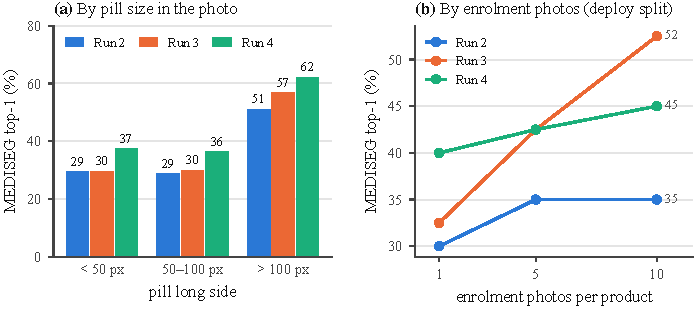
\includegraphics[width=0.92\linewidth,height=0.23\textheight,keepaspectratio]{fig09_robustness.pdf}
  \caption{Robustness on MEDISEG (32 Hong Kong products, other phones, none in training). (a) Top-1 by pill size in the
    photo. (b) MEDISEG's deploy split (40 query pills): more enrolment photos help only partly.}
  \label{fig:robust}
\end{figure}

\begin{figure}[!htbp]
  \centering
  % Match Figure 5's rendered width while preserving this figure's aspect ratio.
  \sbox0{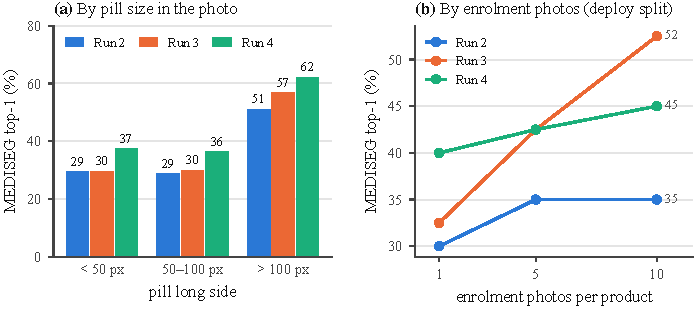
\includegraphics[width=0.92\linewidth,height=0.23\textheight,keepaspectratio]{fig09_robustness.pdf}}
  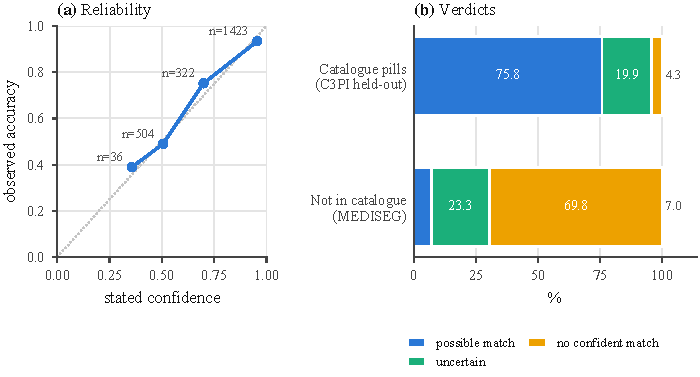
\includegraphics[width=\wd0]{fig13_identify_confidence.pdf}
  \caption{Calibrated confidence for identification. (a) Stated confidence against observed accuracy on held-out
    medicines. (b) Verdicts for catalogue pills and for pills not in the catalogue (MEDISEG).}
  \label{fig:confidence}
\end{figure}

\FloatBarrier
\subsection{Comparison with the ePillID benchmark}
\label{sec:epillid}

The two-sided evaluation averages scores across each front--back pair and includes 626 pairs from 145 types with both sides photographed. The other 47 fold-4 types remain included in the single-photo evaluation; side coverage is shown in Figure~\ref{fig:examples}b.

With one relevant identity per query, MAP corresponds to mean reciprocal rank and MAP@1 to the fraction ranked first. 
In contrast, GAP pools query--candidate scores before calculating average precision, while GAP@1 evaluates top-ranked predictions ordered by score. 
Consequently, a gain in GAP@1 can coexist with lower top-1 accuracy because the measures capture different aspects of ranking and confidence.

Runs 5--7 use the ePillID reference-access setting, permitting references for test types during training while excluding validation groups and types that match their recorded appearance. Retrieval uses the full gallery of 4,902 types (Table~\ref{tab:epillid}).
The embedding alone (MAP 0.57--0.60) falls within the range of the published plain classifiers and remains below the strongest model. 
Re-ranking by imprint, which the paper's model did not use, raises MAP to 0.77--0.78 and GAP@1 to 0.921, above the paper's 0.912, while MAP@1 stays lower (69.0 vs.\ 92.0\%). 
The paper's ablations associate its advantage with its training recipe (contrastive and hard-mined triplet losses with softmax and
ArcFace over side-specific classes, a 2,048-d embedding) alongside its backbone. 
Additional diagnostic comparisons did not recover the gap through crop style, the 64-d pooling step, or local versus global pooling alone.

\begin{table}[!htbp]
  \caption{ePillID benchmark (fold 4, two-sided queries). Runs 5--7 permit test-type references during training but exclude validation groups. The best published model is a ResNet-152 with compact
    bilinear pooling and multi-head metric learning. ``+ imprint'' uses OCR information the published models did not
    use.}
  \label{tab:epillid}
  \centering
  \small
  \begin{tabular}{@{}lccccc@{}}
    \toprule
    & MAP & GAP & MAP@1 & GAP@1 & top-5 \\
    \midrule
    \citet{usuyama2020epillid}, best & \textbf{0.958} & \textbf{0.812} & \textbf{92.0} & 0.912 & -- \\
    \citet{usuyama2020epillid}, plain classifiers & .547--.727 & .241--.448 & 35.7--56.8 & .331--.551 & -- \\
    Ours, run 5 & 0.597 & 0.207 & 45.7 & 0.526 & 77.5 \\
    Ours, run 5 + imprint & 0.780 & 0.598 & 69.0 & \textbf{0.921} & 89.6 \\
    Ours, run 7 + imprint & 0.774 & 0.614 & 67.6 & 0.916 & 89.5 \\
    \bottomrule
  \end{tabular}
\end{table}

\FloatBarrier
\subsection{Error analysis and interpretation}
\label{sec:error-analysis}

\paragraph{Imprint visibility.} A recorded imprint token is recovered on about 47\% of validation photographs, with debossed imprints, small pills and round pills presenting the greatest difficulty. Source visibility labels also identify many unreadable views (Figure~\ref{fig:imprint}), indicating that the available text evidence is constrained by the images themselves.

\paragraph{Look-alike medicines.} When two strengths of one ingredient are enrolled together, one is named as the other in 0.11\% of queries, rising to 0.58\% when shape and colour also match. For pairs sharing an ingredient, the imprint check reduces retakes from 7.5\% to 5.2\% and increases correct naming from 80.1\% to 82.3\%, with a small increase in wrong names. Shared manufacturer prefixes create concentrated errors: tramadol 50\,mg and carvedilol 12.5\,mg are confused in 5.8\% of the corresponding queries despite the imprint check (Figure~\ref{fig:lookalike}). Strength therefore remains associated with the dispensing label rather than confirmed by appearance.

\paragraph{Reader adaptation.} Two LoRA adaptations improve validation imprint recovery from 44.0\% to 53.5\% and from 45.0\% to 50.7\%, respectively. The first produces memorised imprint strings on new pills. The second improves catalogue identification but increases counts of wrong names in the evaluated galleries from 30 to 61. Both adaptations are rejected, as are matching of visually similar characters and separate imprint scoring for each candidate. Full results and representation diagnostics are retained in Appendix~\ref{app:errors}, Table~\ref{tab:negative}.


\FloatBarrier
\section{Conclusion}
PharmaScan combines a learned pill embedding, enrolment prototypes and imprint evidence to verify medicines with explicit rejection and retake decisions. Adaptation of a hybrid facial expression encoder enables enrolment of previously unseen medicines from three photographs. In the strict C3PI evaluation, the gallery using embeddings alone achieves 76.0\% correct naming and 0.04\% accepted misidentification among enrolled queries while rejecting 94.8\% of foreign queries, and imprint re-ranking increases catalogue top-1 accuracy from 71.6\% to 80.2\%. Together, the experiments show that useful embedding separation depends on the training recipe and that improved imprint recovery does not necessarily reduce accepted errors.

Acquisition transfer remains the main limitation because representation learning relies on C3PI consumer images and catalogue coverage is restricted to US products. On MEDISEG, rejection of 70.4\% of enrolled queries limits useful recognition despite rare misidentification among enrolled queries. Small pills and faint or debossed imprints further restrict the available evidence, with an imprint token recovered in about 47\% of validation photographs. The remaining ePillID performance gap and the absence of evaluation on real phone photographs of Singapore medicines and dispensing labels also delimit the current findings.

Future work centres on local enrolment with calibration for each patient or device, evaluating accepted errors alongside rejection and retakes. Controlled branch and fusion comparisons and the ePillID multi-head recipe extend the representation analysis, while adaptation of the imprint reader is assessed through text recovery and downstream verification errors. Prospective studies extend this evaluation to usability and medication errors.

\FloatBarrier
\clearpage
\setlength{\parskip}{5.5pt}
\begingroup
\small
\bibliographystyle{plainnat}
\bibliography{references}
\endgroup
\FloatBarrier
\clearpage
\appendix
\setcounter{figure}{0}
\setcounter{table}{0}
\renewcommand{\thefigure}{A\arabic{figure}}
\renewcommand{\thetable}{A\arabic{table}}
\renewcommand{\theHfigure}{appendix.\arabic{figure}}
\renewcommand{\theHtable}{appendix.\arabic{table}}
\section{Data inventory and qualitative examples}
\label{app:data}
The inventory of consumer images contains 40,587 records, matching the sum of the four partition counts in Table~\ref{tab:data}, whereas 40,550 successful crops are reported. Split generation filters \texttt{crops.csv} to successful detections before assigning partitions and writes \texttt{manifest.csv} and \texttt{summary.json}, but these generated files are absent from the available checkout. Consequently, the available records do not establish whether the discrepancy reflects different preprocessing revisions, and the partition counts remain reported values pending reconciliation with the manifest for the run and crop log.

The MEDISEG inventory similarly distinguishes 14,069 annotated instances from 13,973 evaluated queries. The source paper reports 8,262 images~\citep{chu2026mediseg}, whereas the local retained set contains 8,261. Download and preprocessing records are described in \texttt{epills/docs/datasets.md}. Representative views of the same identity are shown in the main text, Figure~\ref{fig:examples}.


\begin{figure}[!htbp]
  \centering
  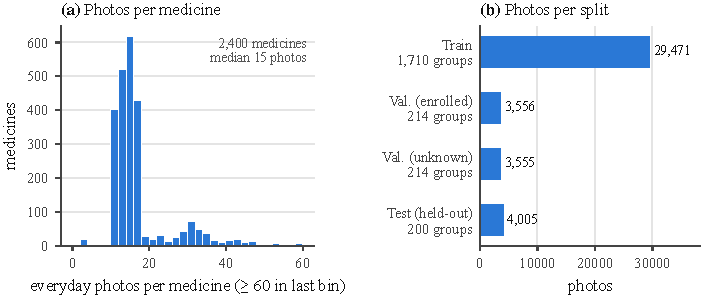
\includegraphics[width=0.94\linewidth,height=0.25\textheight,keepaspectratio]{fig03_data_statistics.pdf}
  \caption{Statistics for C3PI consumer images reproduced from the supplied project materials. (a) Reported images per pill type, defined by NDC9 and product part, with counts of 60 or more pooled in the final bin. (b) Reported partition sizes and counts of appearance groups. Types sharing recorded imprint, shape, colour and size are assigned to the same group, and each group is assigned to one partition. Groups containing an ePillID fold-4 holdout identity form the held-out test partition. The image counts total 40,587 and remain unreconciled with the reported 40,550 successful crops.}
  \label{fig:data-statistics}
\end{figure}

\FloatBarrier
\section{Architecture and training configuration}
\label{app:configuration}
The main training schedule and augmentation are specified in Section~\ref{sec:training}. Table~\ref{tab:arch} lists the layer configuration during inference. Layers after the pretrained backbones use Glorot-uniform initialisation.

\begin{table}[!htbp]
  \caption{The network's layers (inference mode). Pretrained weights: VGG16 on ImageNet, ViT-B/16 on ImageNet-21k.}
  \label{tab:arch}
  \centering
  \small
  \begin{tabular}{@{}p{0.19\linewidth}p{0.62\linewidth}r@{}}
    \toprule
    Block & Details & Output \\
    \midrule
    CNN branch & VGG16 conv.\ blocks $\to$ CBAM $\to$ global average pool $\to$ Dense, ReLU & 256 \\
    ViT branch & ViT-B/16 (\texttt{vit-base-patch16-224-in21k}), pooler output & 768 \\
    Capsule fusion & per branch: Dense 256, ReLU, dropout 0.4, Dense 256, batch norm; dynamic routing, 2 iterations,
      residual update & 256 \\
    Refinement & 4 tokens $\times$ 64 + learned positions; 2 post-norm encoder layers (4 heads, feed-forward width 128, dropout
      0.4); mean pool & 64 \\
    Embedding head & Linear, $\ell_2$ normalisation & 256 \\
    Auxiliary heads & shape (softmax), colour (multi-label sigmoid) & -- \\
    \bottomrule
  \end{tabular}
\end{table}

\FloatBarrier
\section{Calibration and training diagnostics}
\label{app:calibration}
The main evaluation uses rejection, ambiguity and imprint re-ranking parameters selected on validation data. Calibration curves, sequential training changes and training trajectories are collected here to distinguish the selection procedure from the held-out results.

The project plan defines validation targets for a gallery of ten medicines enrolled from three photographs per medicine (Table~\ref{tab:targets}). These are development criteria, not held-out performance claims. In particular, top-1 within the gallery, correct naming at a rejection operating point, and acceptance of foreign queries are distinct measures. Held-out results are reported separately in Table~\ref{tab:main}.

\begin{table}[!htbp]
\centering\small
\caption{Validation targets from the project plan and reported measurements for run 4. These measurements concern validation galleries, with held-out results reported separately.}
\label{tab:targets}
\begin{tabular}{@{}lrr@{}}
\toprule
Measure & Target & Run 4 \\
\midrule
Top-1 within the gallery & $\ge95\%$ & 97.9\% \\
Own-versus-foreign AUROC & $\ge0.90$ & 0.978 \\
Correct naming at 95\% foreign rejection & $\ge80\%$ & 87.9\% \\
Misidentification rate among enrolled queries & $\le 2\%$ & 1.2\% \\
\bottomrule
\end{tabular}
\end{table}

\begin{figure}[!htbp]
  \centering
  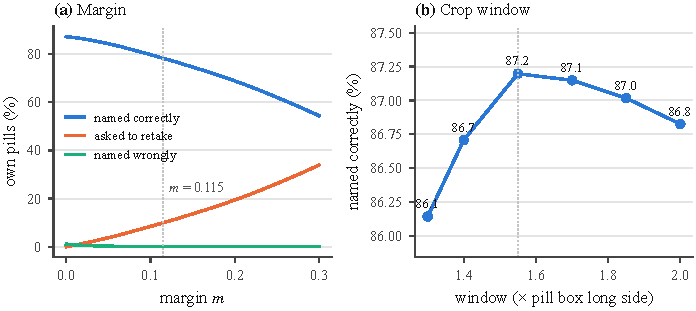
\includegraphics[width=0.92\linewidth,height=0.23\textheight,keepaspectratio]{fig06_calibration.pdf}
  \caption{Settings chosen on validation (1,000 simulated patients, 10 medicines, 3 enrolment photos; $\tau$ rejects
    95\% of other medicines). (a) The margin trades correct names for retakes while wrong names stay near zero.
    (b) Correct naming across crop windows, shown with a narrow $y$-range.}
  \label{fig:calib}
\end{figure}

\begin{table}[!htbp]
  \caption{Sequential design comparisons and parameter sweeps. Multiple changes are combined between runs, so these comparisons do not isolate individual components. Validation results are shown unless a held-out comparison is referenced.}
  \label{tab:ablation}
  \centering
  \small
  \begin{tabular}{@{}p{0.34\linewidth}p{0.46\linewidth}p{0.12\linewidth}@{}}
    \toprule
    Change & Effect & Kept \\
    \midrule
    Run 1$\to$2: lower LRs ($3{\times}10^{-5}$, $10^{-5}$), separate ArcFace LR, margin warm-up & top-1 in 10
      medicines 77.2$\to$98.3\%; AUROC 0.78$\to$0.981; correct at 95\% rejection 17$\to$90.7\%; dims
      $\approx$3$\to$12--15 & yes \\
    Run 2$\to$3: + studio reference photos & validation 98.1\%; higher strict ePillID MAP@1 (Table~\ref{tab:main}) & yes \\
    Run 3$\to$4: + photo and augmentation with crop jitter & higher MEDISEG accuracy with lower C3PI accuracy (Table~\ref{tab:main})
      & yes \\
    Crop window 1.3--2.0$\times$ & named correctly 86.1--87.2\% & 1.55 \\
    Margin $m$ 0--0.3 & named correctly 87$\to$54\%; retakes 0$\to$34\% & 0.115 \\
    Imprint re-ranking $\alpha$, $K$ & top-1 72.1\% ($\alpha{=}0$)$\to$81.6\%; \emph{test} 71.6$\to$80.2\%
      & 0.05, 100 \\
    Gallery check: distinct tokens only & named wrongly 35$\to$30; other pills accepted 6,158$\to$6,150 & yes \\
    Official ePillID protocol (runs 5--7) & ePillID MAP 0.57--0.60; MEDISEG 52--54\% & benchmark \\
    \bottomrule
  \end{tabular}
\end{table}

\begin{figure}[!htbp]
  \centering
  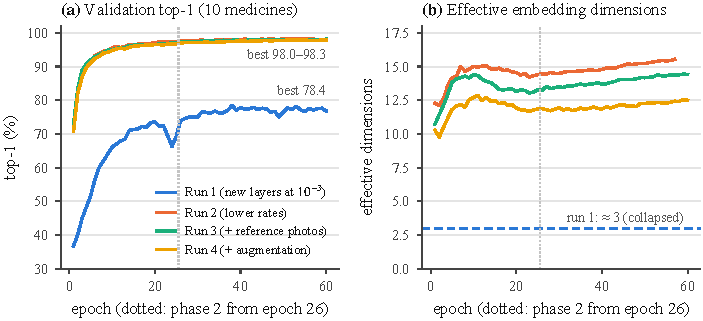
\includegraphics[width=0.92\linewidth,height=0.23\textheight,keepaspectratio]{fig05_training_curves.pdf}
  \caption{Training. (a) Validation top-1 within a gallery of 10 medicines never trained on. (b) Effective embedding
    dimensions: with the new layers at $10^{-3}$ the embedding collapsed to about 3.}
  \label{fig:training}
\end{figure}
\FloatBarrier
\section{Additional error analysis}
\label{app:errors}
\label{sec:errors}

\paragraph{Stratified analysis of imprint reading.} Figure~\ref{fig:imprint} reports validation recovery by recorded imprint type, rater visibility, size and shape. The source analysis uses 7,068 photographs of medicines with a recorded imprint. The corresponding interpretation is given in Section~\ref{sec:error-analysis}.

\begin{figure}[!htbp]
  \centering
  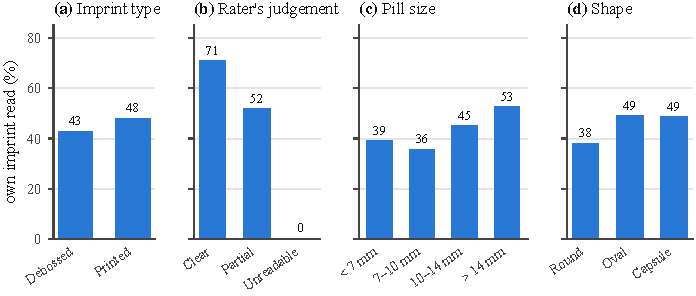
\includegraphics[width=0.92\linewidth,height=0.23\textheight,keepaspectratio]{fig11_imprint_reading.pdf}
  \caption{Share of validation photos on which a token of the pill's own imprint is read (Florence-2-large, zero-shot),
    by imprint type, C3PI rater's judgement of visibility, pill size and shape.}
  \label{fig:imprint}
\end{figure}

\paragraph{Look-alike stress tests.} Both members of each pair are enrolled in the same gallery. Figure~\ref{fig:lookalike} compares matching by appearance alone with the imprint check for different strengths of the same ingredient and pairs from the same manufacturer. The latter share imprint prefixes, including Teva's `TV'. Overall confusion for pairs from the same manufacturer is 0.01\%, but the aggregate masks errors concentrated in individual pairs discussed in Section~\ref{sec:error-analysis}.

\begin{figure}[!htbp]
  \centering
  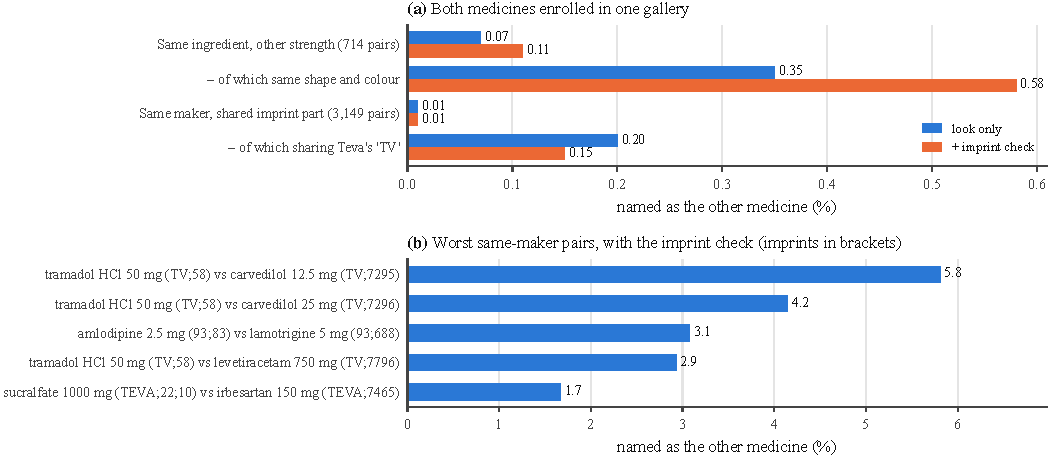
\includegraphics[width=0.92\linewidth,height=0.23\textheight,keepaspectratio]{fig16_lookalike_error_analysis.pdf}
  \caption{Look-alikes, with both medicines enrolled in one gallery. (a) Rates of wrong naming by kind of pair, look only
    and with the imprint check. (b) The worst pairs from the same manufacturer.}
  \label{fig:lookalike}
\end{figure}

\paragraph{Representation diagnostics.} Tracing individual queries yields capsule routing weights of approximately 9\% for the CNN and 91\% for the ViT. Attention between refinement tokens is nearly uniform, describing the feature use observed for these queries. The independent contributions of the branches and fusion mechanism remain unresolved because controlled architectural ablations were not performed.

\paragraph{Rejected variants.} Table~\ref{tab:negative} retains the results of reader adaptation and other rejected variants. Its gallery entries for wrong naming are counts within their respective evaluation configurations, rather than the pooled percentages reported for held-out galleries in Table~\ref{tab:main}.

\begin{table}[!htbp]
  \caption{What did not work (validation).}
  \label{tab:negative}
  \centering
  \small
  \begin{tabular}{@{}p{0.34\linewidth}p{0.46\linewidth}p{0.12\linewidth}@{}}
    \toprule
    Tried & Result & Decision \\
    \midrule
    LoRA of Florence-2-large, v1 (19,312 photos of training medicines) & imprints read 44.0$\to$53.5\%, but
      memorised imprints written onto new pills; identification and gallery check worse & rejected \\
    LoRA v2 (also learns to output nothing on unreadable photos) & own imprint read 45.0$\to$50.7\%; identification
      82.0$\to$83.0\%; gallery wrong names 30$\to$61 & rejected \\
    Look-alike characters (O/0, B/8) treated as equal & measured and dropped & rejected \\
    Scoring each candidate's imprint separately & measured and dropped & rejected \\
    Runs 6--7: stronger fine-tuning; training aligned with the benchmark & better validation and MEDISEG, not ePillID & not
      served \\
    \bottomrule
  \end{tabular}
\end{table}

\FloatBarrier
\section{Implementation and project resources}
\label{app:development}
\label{sec:impl}

The implementation environment reported in the project materials is Python 3.13.15, PyTorch 2.11.0 with CUDA 12.8, and Hugging Face Transformers 5.19.0. Training uses one NVIDIA RTX 4080 SUPER with 16\,GB memory. The pipeline exposes separate stages for partitioning, training, gallery calibration, held-out evaluation, catalogue re-ranking and confidence calibration. The corresponding scripts write configuration, calibration and evaluation records to the run directory.

With the project environment activated, the following PowerShell commands are run from \texttt{epills/}. They reproduce the documented sequence when the required datasets, reference catalogue and cached OCR outputs have been prepared as described in the repository. 

\begin{quote}\small
\begin{verbatim}
$run = 'outputs/runs/stage2_run4'
python scripts/make_splits.py
python scripts/train_stage2.py --config configs/stage2_run4.yaml
python scripts/calibrate_stage2.py --run $run `
  --windows 1.3 1.4 1.55 1.7 1.85 2.0
python scripts/evaluate_stage2.py --run $run
python scripts/tune_identify_rerank.py --run $run --ocr large_c92
python scripts/evaluate_identify_topk.py --run $run --ocr large_c92
python scripts/calibrate_identify.py --run $run --ocr large_c92
python scripts/make_paper_figures.py
\end{verbatim}
\end{quote}

\subsection{Project resources and application prototype}
\label{app:resources}
The image model is deployed through the Hugging Face interface listed in Table~\ref{tab:resources}. A separate care agent application is being developed around this model service, with its deployment and source maintained independently. Its deployment demonstrates application integration in progress. The recognition results in this report evaluate the image pipeline, rather than the agent's medication management behaviour.

\begin{table}[!htbp]
\centering\small
\caption{Project resources supplied by the authors. The care agent application remains under development, and these deployment links document the available demonstrations.}
\label{tab:resources}
\begin{tabular}{@{}p{0.22\linewidth}p{0.73\linewidth}@{}}
\toprule
Resource & Link \\
\midrule
Model demo & \url{https://davidpansx-pharmascan-api.hf.space/ui/} \\
Model source & \url{https://github.com/398-21/ultrasound_Model} \\
Care agent demo & \url{https://medithread.vercel.app} \\
Care agent source & \url{https://github.com/SpectateurLinlan/pharmascan-care-agent} \\
\bottomrule
\end{tabular}
\end{table}

\subsection{Source attribution and report preparation}
The model implementation uses PyTorch and Hugging Face Transformers\footnote{\url{https://github.com/huggingface/transformers}}, with reused project and benchmark code identified in Section~\ref{sec:approach}. The research-paper-writing skill was used for language polishing.

\FloatBarrier
\end{document}
